% !TEX program = xelatex
\documentclass[UTF8,fontset=fandol]{ctexart}

\usepackage[a4paper,top=18mm,bottom=18mm,left=18mm,right=18mm]{geometry}
\usepackage{amsmath,amssymb,bm}
\usepackage{graphicx}
\usepackage{booktabs}
\usepackage{array}
\usepackage{multirow}
\usepackage{makecell}
\usepackage{tabularx}
\usepackage{enumitem}
\usepackage{caption}
\usepackage{float}
\usepackage[section]{placeins}
\usepackage{fancyhdr}
\usepackage{titlesec}
\usepackage{hyperref}
\usepackage[table]{xcolor}

\hypersetup{hidelinks}
\graphicspath{{figures/}}
\setlength{\columnsep}{7mm}
\setlength{\parindent}{2em}
\setlength{\parskip}{0pt}
\setlength{\emergencystretch}{1em}
\setlength{\abovedisplayskip}{4pt}
\setlength{\belowdisplayskip}{4pt}
\setlength{\textfloatsep}{8pt plus 2pt minus 2pt}
\setlength{\floatsep}{7pt plus 2pt minus 2pt}
\setlength{\intextsep}{7pt plus 2pt minus 2pt}
\renewcommand{\arraystretch}{1.08}
\flushbottom

\titleformat{\section}{\bfseries\zihao{4}}{\thesection}{0.6em}{}
\titleformat{\subsection}{\bfseries\zihao{-4}}{\thesubsection}{0.6em}{}
\titlespacing*{\section}{0pt}{8pt}{4pt}
\titlespacing*{\subsection}{0pt}{6pt}{3pt}

\captionsetup{
  font=small,
  labelfont=bf,
  labelsep=quad,
  justification=centering,
  skip=3pt
}
\renewcommand{\figurename}{图}
\renewcommand{\tablename}{表}

\pagestyle{fancy}
\fancyhf{}
\fancyhead[C]{\zihao{-5} 计\ 算\ 机\ 工\ 程 \qquad Computer Engineering}
\fancyfoot[C]{\zihao{-5}\thepage}
\renewcommand{\headrulewidth}{0.4pt}
\renewcommand{\footrulewidth}{0pt}

\newcommand{\method}{GS-OWL}
\newcommand{\osla}{\textsc{OSLA}}
\newcommand{\gws}{\textsc{GWS}}
\newcommand{\placeholder}[1]{\textbf{[待补充：#1]}}
\newcommand{\ppl}{\mathrm{PPL}}
\newcommand{\figsuffix}{color}
\newcommand{\best}[1]{\textbf{#1}}
\newcommand{\second}[1]{\underline{#1}}
\definecolor{paperNavy}{HTML}{17324D}
\definecolor{paperTeal}{HTML}{2A9D8F}
\definecolor{paperOrange}{HTML}{E8843D}
\definecolor{methodRow}{HTML}{E6F4F1}
\definecolor{headerRow}{HTML}{EAF1FA}
\definecolor{ruleGray}{HTML}{AAB4BC}
\arrayrulecolor{black}

\begin{document}
\zihao{-5}

\begingroup
\setlength{\parindent}{0pt}
\begin{center}
{\heiti\zihao{2} GS-OWL：面向大语言模型的双尺度敏感性协同剪枝\par}
\vspace{7pt}
{\zihao{4} \placeholder{第一作者}$^{1}$，\placeholder{第二作者}$^{1}$，\placeholder{第三作者}$^{2,*}$\par}
\vspace{4pt}
{\zihao{-5}
（1.\ \placeholder{单位全称（具体至二级单位），省份 城市 邮编}；
2.\ \placeholder{单位全称（具体至二级单位），省份 城市 邮编}）\par}
\end{center}

\vspace{5pt}
\noindent\textbf{摘\ 要：}
面向资源受限环境的大语言模型训练后非结构化剪枝，需要在给定全局稀疏率下同时决定各层删除量与层内连接位置。统一层稀疏率忽略不同 Transformer 层的可剪性差异，单一连接指标也难以兼顾层间预算和层内排序。为此，提出双尺度敏感性协同剪枝方法 \method。其中，OSLA 以异常比例为锚点，利用相对超阈严重度修正层敏感性，经深度约束和全局预算回投生成非均匀层稀疏率；GWS 将权重幅值与平方根压缩的非负 $L_2$ 聚合梯度结合，在每层预算限定的可行掩码集内执行逐输出行排序。在两种7B模型、3个稀疏率的匹配交叉消融中，OSLA 相对原始 OWL 在12组比较中均降低 WikiText-2 困惑度；固定 OSLA 后，GWS 相对 Wanda 在6组比较中的5组降低困惑度。五个 LLaMA 模型的参数网格结果仅作为测试集择优的候选下包络报告。现有证据支持该方法在所测7B～30B模型、50\%～70\%非结构化稀疏设置中的双尺度互补性；参数稀疏率本身不代表硬件推理加速。

\noindent\textbf{关键词：}
大语言模型；训练后非结构化剪枝；层间预算分配；连接显著性；梯度敏感性；异常值统计

\noindent\textbf{源代码链接：}\placeholder{匿名代码仓库地址；如暂不公开则删除本行}

\noindent 中图分类号：TP391.1 \qquad 文献标志码：A \qquad
DOI：10.19678/j.issn.1000-3428.\placeholder{编辑部分配} \qquad
文章编号：1000-3428（\placeholder{编辑部分配}）

\vspace{8pt}
\begin{center}
{\bfseries\zihao{3} GS-OWL: Dual-Scale Sensitivity Coordination for Post-Training Pruning of Large Language Models\par}
\vspace{5pt}
{\zihao{-4} \placeholder{AUTHOR One}$^{1}$, \placeholder{AUTHOR Two}$^{1}$, \placeholder{AUTHOR Three}$^{2,*}$\par}
\vspace{3pt}
{\zihao{-5}
(1.\ \placeholder{Official School/Department and Institution Name, City Postcode, Province, China};
2.\ \placeholder{Official School/Department and Institution Name, City Postcode, Province, China})\par}
\end{center}

\vspace{4pt}
\noindent\textbf{Abstract:}
Post-training unstructured pruning of large language models for resource-constrained environments must determine both how many connections to remove from each layer and which within-layer connections to remove under a fixed global sparsity target. Uniform layer sparsity ignores differences in prunability across Transformer layers, whereas a single connection metric cannot jointly resolve inter-layer budget allocation and intra-layer ranking. We propose GS-OWL, a dual-scale sensitivity coordination method. OSLA anchors layer sensitivity in the outlier proportion, refines it with relative threshold-exceedance severity, and applies depth constraints and global budget projection to obtain nonuniform layer sparsities. GWS combines weight magnitude with the square root of nonnegative L2-aggregated gradients and performs stable row-wise ranking within the feasible mask set defined by each layer budget. In matched crossed ablations on two 7B models at three sparsity levels, OSLA reduces WikiText-2 perplexity relative to the original OWL allocation in all 12 comparisons; with OSLA fixed, GWS reduces perplexity relative to Wanda in five of six comparisons. Parameter-grid results on five LLaMA models are reported only as test-selected candidate lower envelopes. The available evidence supports complementarity between the two sensitivity scales for the evaluated 7B--30B models under 50\%--70\% unstructured sparsity; parameter sparsity alone does not imply hardware inference speedup.

\noindent\textbf{Key words:}
large language model; post-training unstructured pruning; layer-wise budget allocation; connection saliency; gradient sensitivity; outlier statistics

\vspace{6pt}
\noindent\zihao{-5}
\textbf{基金项目：}\placeholder{基金类别、项目名称及编号}。\quad
\textbf{通信作者：}\placeholder{姓名与长期有效 E-mail}。\quad
\textbf{CCF会员信息：}\placeholder{会员级别及会员号，如无则删除}。
\vspace{4pt}
\endgroup
\vspace{8pt}

\section{引言}

基于 Transformer 的大语言模型（Large Language Model，LLM）通过扩展参数规模、训练数据和计算预算获得了较强的
语言建模与任务迁移能力\cite{llama,llama2,transformer}。与此同时，数十亿至数百亿参数带来的权重存储、显存占用
和数据搬移开销限制了模型在资源受限环境中的部署。剪枝通过移除冗余连接构造稀疏权重，为压缩模型表示和利用稀疏
计算提供基础\cite{obd,obs,han2015,deepcompression}。其中，训练后剪枝仅使用少量校准样本生成掩码，无需恢复
完整预训练过程，适用于预训练数据和计算预算难以复现的大语言模型。

训练后非结构化剪枝包含两个相互关联的决策：在给定全局稀疏预算下确定各 Transformer 层的删除量，以及在层预算
确定后选择需要删除的具体连接。前者决定稀疏预算沿模型深度的分布，后者决定层内掩码位置。SparseGPT\cite{sparsegpt}
利用近似二阶信息和逐列误差补偿降低局部重构误差，Wanda\cite{wanda}根据权重幅值和输入激活能量进行连接排序，
RIA\cite{ria}与 Pruner-Zero\cite{prunerzero}进一步修正或自动构造层内显著性表达式。这类方法主要提高局部连接选择
质量；当各层仍采用统一稀疏率时，层内排序无法补偿敏感层因预算不足而产生的表示扰动。

OWL\cite{owl}利用权重--激活显著性中的异常元素比例描述层间差异，并为异常比例较高的层分配更高保留密度。
该方法以较低统计开销引入非均匀层分配，但其二值计数仅判断元素是否超过均值倍数阈值，未区分轻微超阈与远离阈值的
重尾异常。当两个层具有相近异常比例而异常幅度不同，计数统计会给出近似相同的层重要性。DSA\cite{dsa}、
DLP\cite{dlp}和误差传播分配方法\cite{atp}进一步说明，元素统计的按层归约以及层分数到稀疏率的映射，均是区别于
层内排序的独立决策。因此，仅增强连接显著性或仅使用异常计数，均难以同时处理高稀疏率下的层间预算失配与层内误删。

层内排序还面临敏感信号与优化目标不完全一致的问题。Wanda 的输入激活能量反映通道在校准数据中的使用强度，
但不直接刻画删除单个连接对自回归损失的局部影响。将权重 $W_{ij}$ 置零等价于施加扰动
$\Delta W_{ij}=-W_{ij}$，其一阶损失变化同时受权重和梯度影响。梯度幅值可补充与校准目标相关的局部敏感性，
但直接使用 $\lvert W_{ij}\rvert G_{ij}$ 容易受到重尾聚合梯度支配，并放大有限校准样本引入的排序波动。因此，
连接级指标需要在权重幅值的稳定性与梯度的损失感知能力之间取得平衡。

基于上述分析，本文将训练后非结构化剪枝表述为层间预算与层内连接排序的双尺度协同问题，并提出 \method。
异常严重度感知层分配 OSLA 在异常比例之外引入相对超阈严重度，以异常计数为锚点、尾部幅度为修正量，再通过
深度约束和全局预算回投生成非均匀层稀疏率。梯度加权显著性 GWS 受一阶损失扰动启发，采用
$\lvert W\rvert\sqrt{G}$ 压缩非负聚合梯度的动态范围，并在分配后的层预算内执行逐输出行剪枝。两个模块分别回答
“每层删除多少”和“层内删除哪些”，最终在同一全局稀疏约束下联合生成掩码。

本文主要贡献如下：

1）将训练后非结构化剪枝分解为层间预算与层内排序两个尺度，以层稀疏率 $s_l$ 作为两个模块的预算接口，在固定全局稀疏约束下协同生成掩码。

2）提出异常严重度感知层分配 OSLA，以异常比例为锚点、相对超阈严重度为修正量，经深度约束和预算回投得到满足全局目标的非均匀层稀疏率。

3）提出梯度加权显著性 GWS，用平方根变换压缩聚合梯度的动态范围，并在层预算内逐输出行稳定排序；通过 $2\times3$ 匹配交叉消融分别验证 OSLA 的层间分配作用和 GWS 的层内排序作用。

\section{相关工作}

\subsection{训练后非结构化剪枝与层内决策}

国内研究已从参数剪枝、参数量化、知识蒸馏等路径系统梳理深度模型压缩与加速技术\cite{gao2021compression}，
并进一步总结剪枝粒度、重要性准则及其与结构搜索的关系\cite{mao2023pruning}。
训练后非结构化剪枝的层内决策主要围绕重要性度量、误差补偿和剪枝顺序展开。早期方法利用损失曲率或权重
幅值估计参数重要性\cite{obd,obs,han2015}。面向 LLM，SparseGPT\cite{sparsegpt}将逐层稀疏回归与 Hessian
逆近似结合，在删除权重后更新剩余列以补偿局部重构误差；该方法精度较高，但矩阵分解与逐列补偿增加了计算和显存
开销。Wanda\cite{wanda}使用权重幅值与输入激活能量的乘积进行逐行排序，在不更新权重的条件下降低剪枝成本。
RIA\cite{ria}以行列相对重要性修正绝对幅值偏差，Pruner-Zero\cite{prunerzero}则通过进化搜索自动发现符号化
显著性表达式。上述方法主要改进“层内删除哪些连接”，通常仍在各层采用相同稀疏率。

近期工作进一步研究优化目标和操作次序。FISTAPruner\cite{fistapruner}将逐层剪枝表示为类似 LASSO 的凸优化
问题，并通过累积误差消除支持非结构化和2:4半结构化剪枝。ROSE\cite{rose}指出 SparseGPT 固定的从左到右次序
在列结构明显的权重中可能次优，因而根据列损失和块损失执行两级重排序。这些方法分别从连续优化和误差补偿顺序
提高局部重构质量，但仍需要迭代求解或二阶近似。本文不更新保留权重，也不改变逐层前向流程，而是利用离线聚合
梯度构造连接显著性，并将层间预算作为独立尺度处理。

\subsection{层间稀疏预算分配}

统一层稀疏率实现简单，却默认所有 Transformer 层具有相同的可剪性。OWL\cite{owl}将权重--激活显著性中的
异常元素比例用于层间分配，使异常比例较高的层保留更多连接。AlphaPruning\cite{alphapruning}利用重尾自正则化
理论中的谱形指标估计层质量和可剪性。DSA\cite{dsa}把“元素统计归约为层分数”和“层分数映射为稀疏率”表示为
可搜索运算图，通过进化算法发现分配函数；DLP\cite{dlp}则联合权重与激活信息动态估计层重要性。以上方法从异常
统计、谱分布和自动搜索等不同角度表明，层间异质性是高稀疏率剪枝中不可忽略的因素。

近期研究开始进一步约束分配函数的适用范围。ATP\cite{atp}从跨层误差传播出发推导深度相关的稀疏率，
OptiPrune\cite{optiprune}指出统一分配在较低稀疏率下可能更稳健，而非均匀分配的优势主要出现在较高稀疏率，
并据此调节分配偏差；MRP\cite{mrp}强调层分配应同时考虑指标依赖性和层间冗余均衡。最新的 PALS\cite{pals}
使用激活幅值分位数在有限区间内调整层稀疏率，并报告该收益具有模型依赖性。这些结果说明，层重要性统计、映射函数
和目标稀疏率相互耦合，不能仅凭某个层分数直接推断普适的最优稀疏分布。

不同层分配方法在统计信息与计算代价之间具有不同取舍。OWL 的二值计数开销较低，但丢失异常元素超过阈值的幅度；
谱分析、函数搜索或误差传播可提供更丰富的信息，同时引入额外计算或结构假设。OSLA 保留原始 OWL 的异常比例分配
方向，仅以相对超阈严重度修正尾部差异，并通过有界约束和预算回投满足全局稀疏目标。该设计面向中高稀疏率，
不搜索任意分配函数，而是在异常计数基础上补充可解释的尾部幅度信息。

\subsection{梯度与校准敏感信号}

参数梯度直接关联当前校准目标的一阶损失变化，但其使用方式会影响剪枝成本和稳定性。Wanda++\cite{wandaplusplus}
在解码器块内计算区域梯度，并通过区域优化减小稠密块与稀疏块之间的输出偏差，因此包含剪枝评分和权重优化两个
环节。M-Wanda\cite{mwanda}聚合多语言激活统计并动态调节层稀疏率，说明校准语料分布会改变掩码质量；
DenoiseRotator\cite{denoiserotator}通过旋转集中参数重要性，使现有剪枝器更容易区分保留权重与删除权重。
上述研究表明，重要性信号不仅取决于权重本身，还受到校准数据和参数表示方式的影响。

与 Wanda++ 的区域梯度和权重优化不同，本文只读取校准语料上的聚合梯度，不对模型参数进行恢复或局部更新；
平方根变换用于限制少量极端梯度对排序的支配作用。该梯度仅负责连接级排序，层间分支仍根据权重--激活异常分布
分配预算；这也区别于直接使用梯度幅值决定层稀疏率的方案\cite{pals}。二者在计算与功能上保持解耦，使层分配和
连接显著性的作用能够通过交叉消融分别分析。

此外，LLM-Pruner\cite{llmpruner}、SliceGPT\cite{slicegpt}和 T\'yr-the-Pruner\cite{tyr}通过删除通道、矩阵
切片或结构单元直接缩减稠密计算；GPTQ\cite{gptq}、AWQ\cite{awq}和 LLM.int8()\cite{llmint8}则从数值精度
角度降低存储与矩阵乘开销。国内研究还分别从后训练量化方法体系\cite{zhang2026ptq}、大语言模型推理存储管理
\cite{ge2025storage}以及张量交换与重计算\cite{liang2025adaptive}等方面讨论模型部署效率。本文限定
于 FP16 权重的训练后非结构化剪枝，不把非零参数减少直接等同于端到端加速，也不讨论量化误差或结构恢复训练。

\section{问题定义}

\subsection{训练后非结构化剪枝目标}

设自回归语言模型 $f_{\bm W}$ 含有 $L$ 个 Transformer 解码器块。第 $l$ 个块包含 $J_l$ 个待剪线性权重矩阵，
记为
$\bm W_{l,j}\in\mathbb R^{d_{l,j}^{\mathrm{out}}\times d_{l,j}^{\mathrm{in}}}$，
$j=1,\ldots,J_l$，其集合为
$\mathcal W^{(l)}=\{\bm W_{l,j}\}_{j=1}^{J_l}$。第 $l$ 个块和全模型的待剪参数量分别为
\begin{equation}
n_l=\sum_{j=1}^{J_l}\left|\bm W_{l,j}\right|,
\qquad
N_{\bm W}=\sum_{l=1}^{L}n_l .
\label{eq:parameter_count}
\end{equation}
给定由 $N_c$ 个序列构成的校准集
$\mathcal D_c=\{\bm x^{(n)}\}_{n=1}^{N_c}$，校准目标采用序列平均自回归负对数似然：
\begin{equation}
\mathcal L_c(\bm W)
=
-\frac{1}{\sum_{n=1}^{N_c}T_n}
\sum_{n=1}^{N_c}\sum_{t=1}^{T_n}
\log p_{\bm W}\!\left(x_t^{(n)}\mid \bm x_{<t}^{(n)}\right).
\label{eq:calibration_loss}
\end{equation}

对每个权重矩阵引入同形二值掩码
$\bm B_{l,j}\in\{0,1\}^{d_{l,j}^{\mathrm{out}}\times d_{l,j}^{\mathrm{in}}}$，
其中0表示删除连接，1表示保留连接。剪枝后的权重为
$\widetilde{\bm W}_{l,j}=\bm W_{l,j}\odot\bm B_{l,j}$，且所有保留权重保持原值。对于目标稀疏率
$s\in[0,1)$，实际需要删除的整数参数量记为
$K=\operatorname{round}(sN_{\bm W})$。训练后非结构化剪枝的理想目标为
\begin{equation}
\begin{aligned}
\min_{\{\bm B_{l,j}\}}\quad&
\mathcal L_c(\bm W\odot\bm B),\\
\mathrm{s.t.}\quad&
\sum_{l=1}^{L}\sum_{j=1}^{J_l}
\left\|\bm 1-\bm B_{l,j}\right\|_0=K,\\
&\bm B_{l,j}\in\{0,1\}^{d_{l,j}^{\mathrm{out}}\times d_{l,j}^{\mathrm{in}}}.
\end{aligned}
\label{eq:objective}
\end{equation}
式(\ref{eq:objective})限定保留权重不经微调或重构，因此优化变量仅为二值掩码。由于搜索空间随
$N_{\bm W}$ 指数增长，该离散优化问题无法在十亿参数模型上直接求解。

\subsection{层间预算与层内排序的双尺度分解}

令第 $l$ 个块的删除量为
$k_l=\sum_j\|\bm 1-\bm B_{l,j}\|_0$，对应层稀疏率和保留密度分别为
$s_l=k_l/n_l$ 与 $d_l=1-s_l$。所有可行层预算构成集合
\begin{equation}
\mathcal S(s)=
\left\{
\bm s\in[0,1)^L:
\sum_{l=1}^{L}n_ls_l=K,\ 
n_ls_l\in\mathbb Z_{\geq 0}
\right\}.
\label{eq:layer_budget_set}
\end{equation}
当各解码器块包含相同数量的待剪参数时，式(\ref{eq:layer_budget_set})退化为
$L^{-1}\sum_l s_l\approx s$；统一剪枝进一步限制所有 $s_l=s$。给定某个
$\bm s\in\mathcal S(s)$，记 $\mathcal B(\bm s)$ 为每个块恰好删除 $k_l$ 个连接的掩码集合，则
式(\ref{eq:objective})可等价写成
\begin{equation}
\min_{\bm s\in\mathcal S(s)}
\quad
\min_{\bm B\in\mathcal B(\bm s)}
\mathcal L_c(\bm W\odot\bm B).
\label{eq:nested_objective}
\end{equation}
外层变量 $\bm s$ 回答“每层删除多少”，内层变量 $\bm B$ 回答“层内删除哪些”。外层估计偏差可能使敏感层承担
过多删除量，内层排序偏差则会在既定预算内误删关键连接，因而两个子问题不能由单一排序分数相互替代。

训练后方法通常用可计算的代理量近似上述两层组合优化。设
$z_l=\Phi(\mathcal W^{(l)},\mathcal D_c)$ 为第 $l$ 个块的统计量，
$M_{l,j,r,c}=\mathcal R(\bm W_{l,j},\mathcal D_c)$ 为连接级显著性，则双尺度剪枝可表示为
\begin{equation}
\bm s=\mathcal A(\bm z;s,\Theta_A),
\qquad
\bm B=\mathcal T(\bm M,\bm s),
\label{eq:dual_scale_mapping}
\end{equation}
其中 $\mathcal A$ 将层统计映射为满足式(\ref{eq:layer_budget_set})的预算，
$\mathcal T$ 则在预算内删除低显著性连接。本文采用逐输出行剪枝：若第 $(l,j)$ 个矩阵每行包含
$d_{l,j}^{\mathrm{in}}$ 个连接，则第 $r$ 行删除
$q_{l,j}=\lfloor s_ld_{l,j}^{\mathrm{in}}\rfloor$ 个最小显著性元素，
\begin{equation}
B_{l,j,r,c}
=
\mathbb I\!\left[
\operatorname{rank}_{\uparrow}
\!\left(M_{l,j,r,c}\right)>q_{l,j}
\right],
\label{eq:rowwise_mask}
\end{equation}
其中 $\operatorname{rank}_{\uparrow}$ 表示在同一输出行内按升序进行稳定排序。逐行约束避免某些输出通道独占保留
预算，也使不同矩阵只需共享层稀疏率而无需直接比较显著性绝对尺度。若所有行均向下取整，离散化后的总删除量
$\widehat K$ 满足 $0\leq K-\widehat K<R_{\mathrm{row}}$，其中 $R_{\mathrm{row}}$ 为待剪矩阵的输出行总数；
因此实验除目标稀疏率外还需报告实际稀疏率。

在上述形式化框架下，层间统计 $\Phi$ 与连接排序 $\mathcal R$ 无需采用同一种信号：前者描述整个块的相对可剪性，
后者区分块内连接的相对重要性。第4章分别以权重--激活异常分布实现 $\Phi$ 和 $\mathcal A$，以经动态范围压缩的
聚合梯度实现 $\mathcal R$，并通过全局预算投影使两个尺度共同生成满足目标稀疏率的掩码。

\section{GS-OWL 双尺度敏感协同剪枝方法}

方法的整体结构、双分支信息流与预算接口如图\ref{fig:overview}所示。

\FloatBarrier
\begin{figure*}[t]
  \centering
  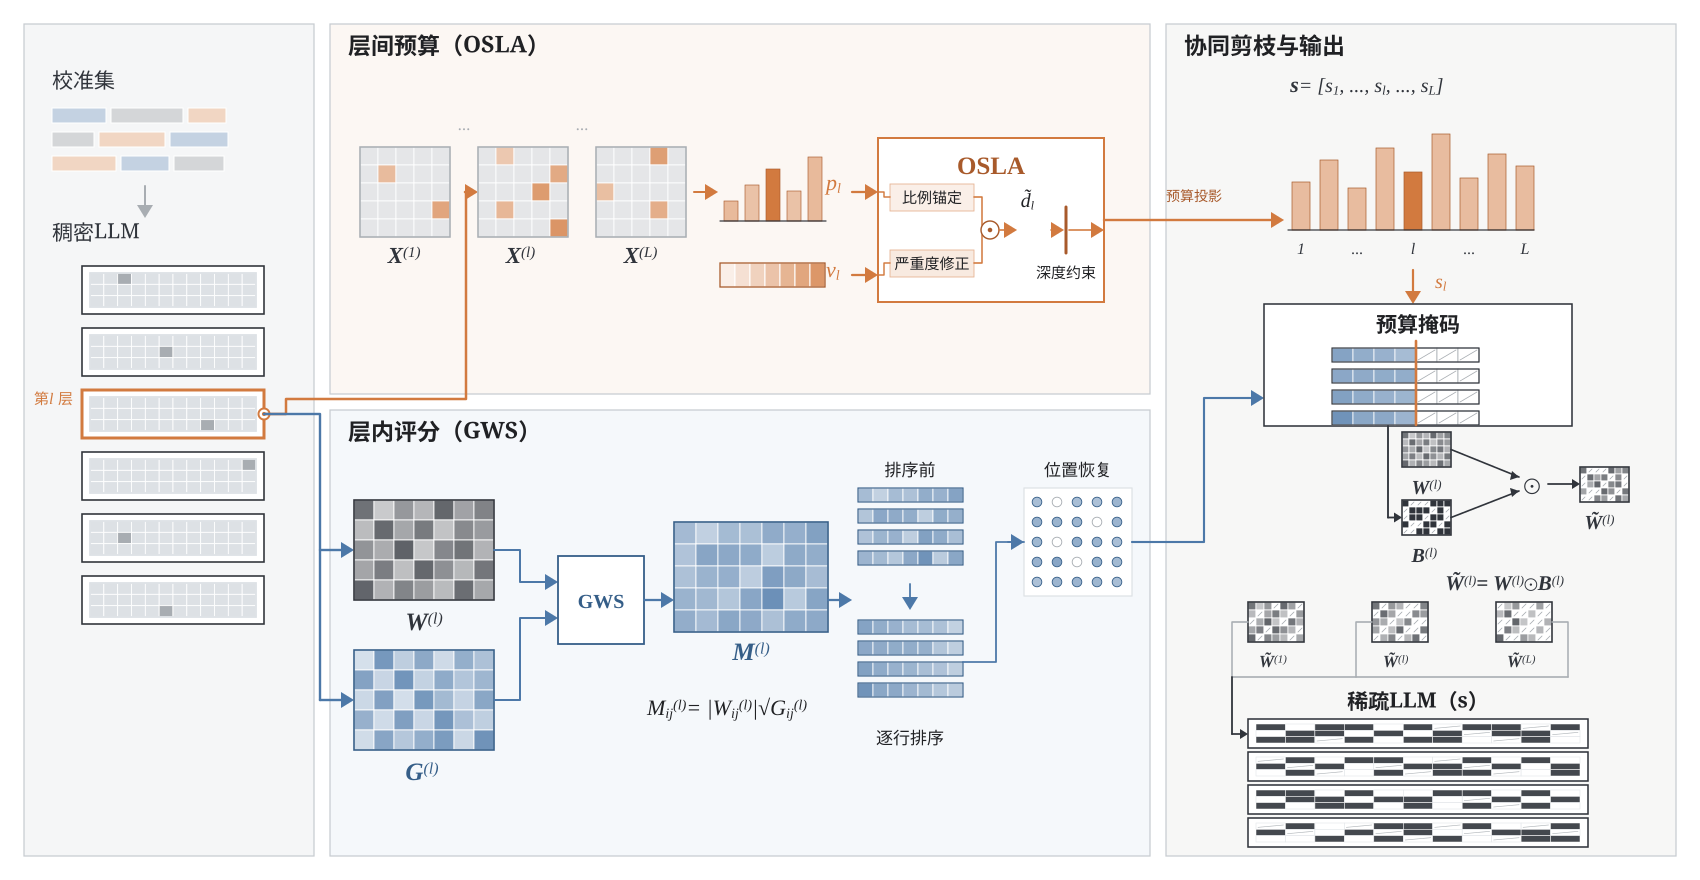
\includegraphics[width=0.99\textwidth]{GS_OWL_framework_strict_review.pdf}
  \caption{GS-OWL 双尺度敏感协同框架：OSLA 估计层间预算，GWS 在预算约束下生成逐行连接掩码\\
  Fig. 1 Dual-scale sensitivity coordination in GS-OWL: OSLA estimates layer-wise budgets and GWS generates row-wise connection masks}
  \label{fig:overview}
\end{figure*}

\subsection{总体框架}

在该框架中，\method 不使用单一分数同时完成层间分配和层内选择，而是分别估计层间敏感性与连接级
显著性，并以层稀疏率为接口耦合两个模块。给定预训练权重 $\bm W$、目标全局稀疏率 $s$、激活校准集
$\mathcal D_X$ 和梯度校准集 $\mathcal D_G$，层间分支先从权重--激活异常分布中提取异常比例
$\bm p=[p_1,\ldots,p_L]$ 和超阈严重度 $\bm v=[v_1,\ldots,v_L]$，经计数锚定融合、深度约束和预算回投得到
层预算向量 $\bm s=[s_1,\ldots,s_l,\ldots,s_L]$。连接级分支由权重和离线聚合梯度生成显著性矩阵 $\bm M$，
并在第 $l$ 个块的预算 $s_l$ 下逐输出行产生二值掩码。整体映射可概括为
\begin{equation}
\begin{aligned}
\bm d&=\Pi_s\!\left(
\mathcal C_{\mathrm{dep}}\!\left[
(1-\alpha)\mathcal A(\bm p)+\alpha\mathcal A(\bm v)
\right]\right),\\
\bm s&=\bm 1-\bm d,\qquad
\bm B=\mathcal T\!\left(\mathcal R(\bm W,\bm G),\bm s\right),
\end{aligned}
\label{eq:framework}
\end{equation}
其中，$\mathcal A$ 为层统计到保留密度的有界映射，$\mathcal C_{\mathrm{dep}}$ 为深度约束，$\Pi_s$ 为全局预算
回投，$\mathcal R$ 和 $\mathcal T$ 分别表示连接显著性计算与逐行截断。$\mathcal D_X$ 和 $\mathcal D_G$ 均只用于
统计估计，可以相同，也可以分别离线构造；梯度张量生成后可复用于不同目标稀疏率。最终仅将掩码乘到预训练权重上，
不更新保留权重，也不进行稀疏模型微调。

该分解便于区分两类误差来源：若 $s_l$ 过大，敏感层获得的保留容量不足，层内排序无法补偿预算缺失；若
$\bm M$ 的局部排序失真，即使层预算合理，仍可能在块内删除关键连接。因此，\method 不将两类信号直接混合为
全局分数，而是使每类信号处理与其统计粒度相匹配的子问题。这里的“协同”并非将 OWL 与梯度分数简单串联：
$s_l$ 同时限定 GWS 的可行掩码集合和每个输出行的精确删除配额，GWS 只能在 OSLA 分配的预算内改变连接位置。

\noindent\textbf{主要符号：}\par
\begin{center}
\footnotesize
\setlength{\tabcolsep}{3.2pt}
\renewcommand{\arraystretch}{0.96}
\begin{tabular}{p{0.18\columnwidth}p{0.28\columnwidth}p{0.18\columnwidth}p{0.28\columnwidth}}
\toprule
符号 & 含义 & 符号 & 含义 \\
\midrule
$s,\ \bm s$ & 全局稀疏率与层预算向量 & $s_l,\ d_l$ & 第$l$层稀疏率与保留密度 \\
$p_l,\ v_l$ & 异常比例与严重度加权比例 & $\widetilde d_l,\widehat d_l$ & 融合密度与约束后密度 \\
$\bm W^{(l)},\bm G^{(l)}$ & 第$l$层权重与聚合梯度 & $\bm M^{(l)},\bm B^{(l)}$ & 显著性矩阵与二值掩码 \\
$\mathcal D_X,\mathcal D_G$ & 激活与梯度校准集 & $N_b,\ q_{l,j}$ & 梯度小批次数与逐行删除数 \\
\bottomrule
\end{tabular}
\end{center}

\subsection{梯度加权连接显著性 GWS}

\subsubsection*{1）一阶扰动与离线梯度聚合}

对于任意线性权重 $W_{ij}^{(l)}$，将其删除等价于施加扰动
$\Delta W_{ij}^{(l)}=-W_{ij}^{(l)}$。在预训练参数附近对校准损失进行一阶展开，有
\begin{equation}
\Delta\mathcal L_{ij}^{(l)}
\approx
\frac{\partial\mathcal L}{\partial W_{ij}^{(l)}}
\Delta W_{ij}^{(l)}
=-W_{ij}^{(l)}g_{ij}^{(l)} .
\label{eq:taylor}
\end{equation}
式(\ref{eq:taylor})说明，权重幅值与有符号损失梯度共同影响单连接的一阶局部扰动。然而，单个序列或小批次梯度容易受
token 组成影响，直接用于排序会产生较大波动。设训练语料子集 $\mathcal D_G$ 被划分为 $N_b$ 个小批次，第 $b$ 个小批次的
自回归损失为 $\mathcal L_b$，本文按元素进行 $L_2$ 聚合：
\begin{equation}
G_{ij}^{(l)}
=
\left[
\sum_{b=1}^{N_b}
\left(
\frac{\partial\mathcal L_b}{\partial W_{ij}^{(l)}}
\right)^2
\right]^{1/2}.
\label{eq:gradient_aggregation}
\end{equation}
由定义可知，$G_{ij}^{(l)}\geq0$，它反映多个小批次上的梯度幅值而不保留方向，因此不等同于完整语料总损失的
有符号梯度。实现中的统一梯度缩放常数只改变所有元素的共同尺度，不改变同一权重矩阵内的排序，因此式
(\ref{eq:gradient_aggregation})省略该常数。聚合结果以半精度张量离线保存，剪枝时按层和模块读取。

\subsubsection*{2）平方根动态范围压缩}

式(\ref{eq:taylor})启发的直接幅值代理可写为 $\lvert W_{ij}^{(l)}\rvert G_{ij}^{(l)}$，但聚合梯度仍具有明显长尾：
少数极大梯度可能掩盖权重幅值差异，并放大有限训练样本带来的排序噪声。为在梯度敏感性与权重尺度之间取得更平缓的平衡，定义
\begin{equation}
M_{ij}^{(l)}
=
\left|W_{ij}^{(l)}\right|
\sqrt{G_{ij}^{(l)}}.
\label{eq:gws}
\end{equation}
式(\ref{eq:gws})对非负 $L_2$ 聚合梯度幅值施加$1/2$指数，同时保留权重幅值的一次尺度。$M_{ij}^{(l)}$ 越大，
表示该连接在当前代理指标下具有越高的保留优先级。平方根变换用于经验性地压缩动态范围，不构成离散剪枝损失的
精确一阶估计或严格二阶近似。

对于第 $l$ 个块中第 $j$ 个权重矩阵，每个输出行删除
$q_{l,j}=\lfloor s_l d_{l,j}^{\mathrm{in}}\rfloor$ 个最低分元素，掩码按式(\ref{eq:rowwise_mask})生成。逐行约束使各输出
通道共享同一层预算，避免尺寸较大的模块或少数行通过绝对分数尺度占用大部分删减名额；稳定排序还保证相同输入和
参数下的掩码可复现。

\subsection{异常严重度感知层分配 OSLA}

\subsubsection*{1）异常数量与超阈严重度}

层间分支以 OWL\cite{owl} 的权重--激活异常证据为基础。对于第 $l$ 个解码器块的第 $j$ 个线性模块，输入通道
$c$ 的激活能量记为 $X_{l,j,c}$，元素级异常得分为
\begin{equation}
O_{l,j,r,c}
=
\left|W_{l,j,r,c}\right|\sqrt{X_{l,j,c}} .
\label{eq:outlier}
\end{equation}
将同一块内所有线性模块的 $\bm O_{l,j}$ 展平并拼接为向量 $\bm o_l$，以
$\tau_l=H_m\operatorname{mean}(\bm o_l)$ 作为自适应阈值。原始 OWL 使用超过阈值的元素比例描述层异常程度：
\begin{equation}
p_l
=
\frac{1}{n_l}
\sum_{u=1}^{n_l}\mathbf 1(o_{l,u}>\tau_l).
\label{eq:count}
\end{equation}
$p_l$ 能够回答“异常元素有多少”，却不能区分轻微越过阈值和远高于阈值的异常尾部。为补充幅度信息，定义平均相对
超阈量 $e_l$ 和严重度加权比例 $v_l$：
\begin{equation}
\begin{aligned}
e_l&=
\frac{1}{m_l}
\sum_{u:o_{l,u}>\tau_l}
\frac{o_{l,u}-\tau_l}{\tau_l+\varepsilon},
\qquad
m_l=\sum_{u=1}^{n_l}\mathbf 1(o_{l,u}>\tau_l),\\
v_l&=p_l\left[1+\log(1+e_l)\right].
\end{aligned}
\label{eq:severity}
\end{equation}
若 $m_l=0$，则令 $e_l=v_l=0$。由于 $v_l$ 以 $p_l$ 为基线，异常尾部整体远离阈值时才会提高对应层的
敏感性估计；对数函数用于限制少量极端值造成的过度修正。

\subsubsection*{2）计数锚定的密度映射}

对任意层统计向量 $\bm q=[q_1,\ldots,q_L]$，先计算
\begin{equation}
z_l(\bm q)=
\begin{cases}
\dfrac{q_l-\min_k q_k}{\max_k q_k-\min_k q_k},
& \max_k q_k>\min_k q_k,\\[6pt]
0,&\text{其他},
\end{cases}
\label{eq:minmax}
\end{equation}
再将高统计量映射为低稀疏率：
\begin{equation}
\begin{aligned}
\bar s_l(\bm q)
&=\operatorname{clip}\!\left(
s+\lambda[1-2z_l(\bm q)],\,
\underline s,\overline s\right),\\
d_l(\bm q)&=
1-\operatorname{clip}\!\left(
\bar s_l(\bm q)-[\operatorname{mean}(\bar{\bm s})-s],\,
\underline s,\overline s\right),
\end{aligned}
\label{eq:density_mapping}
\end{equation}
其中 $\underline s=\max(0.01,s-\lambda)$，$\overline s=\min(0.99,s+\lambda)$。式
(\ref{eq:density_mapping})先限制单层偏移，再在可行边界内校正候选稀疏率均值。分别代入 $\bm p$ 和 $\bm v$，
得到比例密度 $\bm d^p$ 与严重度密度 $\bm d^v$。OSLA 不以严重度分支替代原始比例分支，而采用
\begin{equation}
\widetilde d_l=(1-\alpha)d_l^p+\alpha d_l^v .
\label{eq:fusion}
\end{equation}
本文将融合系数限制为 $\alpha\in[0.10,0.25]$，使计数密度的权重不低于75\%，严重度分支仅用于修正异常幅度。
该锚定方式保留原始 OWL 的主要分配方向，并降低单独采用尾部统计时对极端层过度保护的风险。

\subsubsection*{3）深度约束与全局预算回投}

为限制严重度分支在深度方向上造成局部分配反转，本文为中前部核心区
$\mathcal C=\{5,\ldots,11\}$ 设置密度下界，并为中后段区 $\mathcal T=\{17,\ldots,31\}$ 设置密度上界；
区间按1起始层编号表示，超出模型深度的部分自动截断，代码中的0起始索引分别为4--10和16--30。约束后的候选密度为
\begin{equation}
\widehat d_l=
\begin{cases}
\max(\widetilde d_l,d_l^p), & l\in\mathcal C,\\
\min(\widetilde d_l,d_l^p), & l\in\mathcal T,\\
\widetilde d_l, & \text{其他}.
\end{cases}
\label{eq:depth_constraints}
\end{equation}
核心区不允许严重度分支将保留密度降至计数基线以下，中后段区不允许其将保留密度提高至计数基线以上。该非对称约束
用于抑制严重度修正造成的局部分配反转，不表示所有模型架构均具有相同的理论最优层区间。

最后，将 $\widehat{\bm d}$ 回投到有界预算集合
\begin{equation}
\mathcal Q_s=
\left\{
\bm d:
d_l\in[1-\overline s,1-\underline s],\
\frac{1}{L}\sum_{l=1}^{L}(1-d_l)=s
\right\},
\qquad
\bm d=\Pi_s(\widehat{\bm d}),\qquad s_l=1-d_l.
\label{eq:budget}
\end{equation}
预算回投根据各层到边界的剩余容量迭代分配密度差额；当总密度需要下降时，优先使用非核心层的可用容量，若容量不足
再放宽到全部层。对于本文测试的 decoder-only 模型，每个解码器块包含相同数量的待剪参数，因此式
(\ref{eq:budget})与第3章的参数加权全局预算等价。逐行整数取整仍会产生小于输出行总数的离散误差，故实验部分
继续报告实测稀疏率。

\subsection{协同掩码生成}

\noindent\textbf{算法1 GS-OWL掩码生成流程}\par
\noindent\textbf{输入：}预训练模型 $\bm W$，目标全局稀疏率 $s$，校准集 $\mathcal D_X,\mathcal D_G$，
异常阈值倍数 $H_m$、预算范围 $\lambda$、融合系数 $\alpha$、深度约束区间 $\mathcal C,\mathcal T$
及梯度指数 $\beta=1/2$。\par
\noindent\textbf{输出：}二值掩码 $\bm B$、稀疏权重 $\widetilde{\bm W}=\bm W\odot\bm B$ 及实测全局稀疏率。\par
\begin{enumerate}[leftmargin=2.3em,itemsep=2pt,topsep=2pt]
  \item 在 $\mathcal D_X$ 上逐块传播激活并累计输入通道能量，由式(\ref{eq:outlier})--式(\ref{eq:severity})
  计算每层异常比例 $p_l$ 与严重度加权比例 $v_l$。
  \item 分别映射 $\bm p$ 与 $\bm v$ 得到 $\bm d^p,\bm d^v$，按式(\ref{eq:fusion})融合为
  $\widetilde{\bm d}$，再施加式(\ref{eq:depth_constraints})的核心区下界和中后段上界。
  \item 通过式(\ref{eq:budget})回投并修正预算，得到最终保留密度 $\bm d$ 与
  $\bm s=\bm 1-\bm d$；逐层记录 $s_l$。
  \item 在 $\mathcal D_G$ 的 $N_b$ 个小批次上按式(\ref{eq:gradient_aggregation})聚合梯度，离线保存
  $\bm G^{(l)}$；剪枝时按层读取并由式(\ref{eq:gws})计算 $\bm M^{(l)}$。
  \item 对第$l$层第$j$个权重矩阵的每个输出行执行稳定升序排序，删除最低的
  $q_{l,j}=\lfloor s_l d_{l,j}^{\mathrm{in}}\rfloor$ 个连接并生成 $\bm B^{(l,j)}$。
  \item 写入 $\widetilde{\bm W}^{(l,j)}=\bm W^{(l,j)}\odot\bm B^{(l,j)}$，将当前块输出传给下一块；
  完成全部块后，以零权重计数核验实际全局稀疏率。
\end{enumerate}
步骤1--3只确定“每层剪多少”，步骤4--6只确定“层内剪哪些”；二者通过 $s_l$ 单向耦合，因而可以在不改变
OSLA 的情况下替换连接显著性，也可以固定 \gws 对层预算方法进行独立消融。

\subsection{复杂度与工程边界}

设待剪参数总数为 $P$，最大输入维度为 $d_{\max}$，第 $l$ 个块的参数量为 $P_l$。在聚合梯度已离线生成的条件下，
异常得分、\gws 显著性和掩码写入均为 $O(P)$ 的逐元素操作，逐输出行排序的最坏时间复杂度为
$O(P\log d_{\max})$。层统计阶段和剪枝阶段各需要一次校准激活传播；梯度生成则额外需要在 $\mathcal D_G$ 上执行
反向传播，但同一梯度文件可以复用于多个稀疏率设置。

离线梯度文件的最坏存储复杂度为 $O(P)$。实现中梯度常驻 CPU 并按层搬移，设备侧主要保存当前层的
$O(P_l)$ 显著性、掩码和校准激活缓存，避免同时保留全模型显著性矩阵。相较 Wanda，\method 的主要附加成本是
梯度生成、存储和读取；相较 SparseGPT，其不构造输入维度平方级的 Hessian 近似，也不执行逐列权重重构。
上述复杂度仅描述掩码生成过程。非结构化零权重能否转化为端到端推理加速，仍取决于稀疏算子、硬件后端和存储格式，
本文不将参数稀疏率直接等同于通用 GPU 上的加速比。

\section{实验与结果分析}

本节从语言建模质量、候选集合覆盖、组件归因、稳健性、迁移趋势和领域候选覆盖6个方面评估 \method：1）不同模型和稀疏率下的
WikiText-2 困惑度；2）已评测稀疏掩码集合对不同零样本任务的覆盖情况；3）OSLA 与 GWS 对层间预算和层内排序的
作用；4）方法对随机种子和校准样本数的敏感性；5）模型架构、微调模型及评价语料变化下的结果趋势；6）PLLaMA
领域模型候选掩码集合在植物科学选择题上的 oracle 覆盖上界。除特别说明外，所有结果均来自训练后
非结构化剪枝，掩码生成后不再更新保留权重。

\subsection{实验设置}

\textbf{模型与剪枝设置：}主实验采用 LLaMA-1-7B/13B/30B 和 LLaMA-2-7B/13B，扩展实验采用 Mistral-7B 和 Vicuna-7B，
分别考察不同解码器架构和指令微调模型上的表现；领域任务实验采用 PLLaMA-7B-base 和 PLLaMA-13B-base。
模型规模覆盖7B～30B。所有模型以 FP16 加载，仅剪除解码器块中的线性层权重，词嵌入、归一化层与语言模型输出头
保持稠密。目标稀疏率设置为 $s\in\{0.50,0.60,0.70\}$，实际稀疏率由待剪权重中的零元素比例重新计算；
所有有效主实验的实测值与目标值之差均不超过0.0005。

\textbf{校准数据与评价指标：}本文区分激活校准集 $\mathcal D_X$ 与梯度校准集 $\mathcal D_G$。激活统计由
C4\cite{c4} 训练集估计，默认使用128个长度为2\,048的序列，随机种子为0；连接级梯度由 WikiText-2 训练集序列
按小批次计算并以 $L_2$ 形式离线聚合，剪枝阶段只读取对应张量。语言建模性能采用
WikiText-2\cite{wikitext} 测试集 PPL，数值越低越好。零样本评测基于 lm-evaluation-harness 的零样本（0-shot）协议，包含
BoolQ\cite{boolq}、RTE\cite{glue}、HellaSwag\cite{hellaswag}、ARC-Challenge、ARC-Easy\cite{arc}、WinoGrande\cite{winogrande}
和 OpenBookQA\cite{openbookqa}。HellaSwag 与 OpenBookQA 报告归一化准确率（acc\_norm），其余任务报告准确率
（acc），数值越高越好。除 WikiText-2 测试集外，本文还将由 WikiText-2 主实验确定的固定配置迁移至 C4 验证集，
用于检查评价语料变化下的 PPL 表现，不在 C4 上重新选择配置。PPL 与下游准确率衡量不同能力，本文分别报告，
不以其中一项替代另一项。

\textbf{对比方法：}选取 Dense FP16 参考模型以及 Magnitude、Wanda、SparseGPT、RIA 和 Pruner-Zero 剪枝方法。Magnitude 提供
无校准幅值基线；Wanda 与 SparseGPT 分别代表激活感知排序和近似二阶重构；RIA 与 Pruner-Zero 代表相对重要性
修正和自动显著性搜索。除标注为公开文献参考值的结果外，其余基线均采用与本文一致的模型、稀疏率和评价协议。
严格消融使用 Wanda/GWS 与均匀分配/原始 OWL/OSLA 的 $2\times3$ 交叉组合，
从而分别控制层内排序和层间预算变量。

\textbf{候选选择协议：}主表中每个模型--稀疏率组合评测120个配置：
$H_m\in\{5,6,7\}$，$\lambda\in\{0.02,0.04,\ldots,0.20\}$，
$\alpha\in\{0.10,0.15,0.20,0.25\}$，激活校准随机种子固定为0。现有实验没有独立验证集，
配置由同一 WikiText-2 测试集 PPL 选择，因此 \method 数值只能解释为候选配置的测试集下包络，不能作为预先固定配置的
无偏测试结果，也不参与与单配置基线的最优/次优排名。扩展模型结果采用各自已评测候选集合的最低 PPL，同样按探索性
下包络处理。稳健性、效率和 C4 跨语料分析采用固定配置。零样本表报告逐任务 oracle 上包络；PLLaMA 每个稀疏率
评测20个候选掩码，并在同一565题集合上选择和报告最高准确率，二者均不作为单一固定掩码的泛化证据。

\textbf{实现与统计：}实验主要使用 PyTorch 2.6.0、Transformers 4.36.2--4.37.2 和 Accelerate 1.10.1，
在 NVIDIA A40、A100 与 L20 GPU 上完成。每次运行
保存完整配置、实际稀疏率、剪枝时间以及逐层保留密度和稀疏率；统计仅纳入完成全部剪枝与评测流程的有效结果。
稳定性实验报告3个随机种子的均值与样本标准差。Dense FP16 数值采用公开文献中的同模型参考值并以
$\dagger$ 标注。时间对比仅使用相同 A40 环境下、给定离线梯度后的掩码生成测量结果。

\subsection{WikiText-2 语言建模结果}

表\ref{tab:ppl}按稀疏率分组报告5个 LLaMA 主模型的 WikiText-2 PPL。

\begin{table}[!htbp]
\centering
\caption{5个 LLaMA 模型的固定基线结果与 GS-OWL 候选配置测试集下包络（WikiText-2 PPL$\downarrow$）\\
Table 1 Fixed-baseline results and test-selected GS-OWL candidate lower envelopes on five LLaMA models (WikiText-2 PPL$\downarrow$)}
\label{tab:ppl}
\scriptsize
\setlength{\tabcolsep}{4.2pt}
\renewcommand{\arraystretch}{0.96}
\begin{tabular*}{0.98\textwidth}{@{\extracolsep{\fill}}lcrrrrr@{}}
\toprule
\multirow{2}{*}{方法} & \multirow{2}{*}{稀疏率} &
\multicolumn{3}{c}{LLaMA-1 / PPL$\downarrow$} & \multicolumn{2}{c}{LLaMA-2 / PPL$\downarrow$} \\
\cmidrule(lr){3-5}\cmidrule(lr){6-7}
 & & 7B & 13B & 30B & 7B & 13B \\
\midrule
Dense FP16$\dagger$ & 0\% & 5.6700 & 5.0900 & 4.7700 & 5.4700 & 4.8800 \\
\midrule
Magnitude & \multirow{6}{*}{50\%} & 17.2600 & 20.1300 & 7.5400 & 16.0300 & 6.8200 \\
Wanda & & 7.2500 & 6.5700 & 5.2400 & 7.7800 & 6.2800 \\
SparseGPT & & 7.2000 & 6.2000 & 5.3100 & 6.5100 & 5.6200 \\
RIA & & \second{7.1200} & \second{6.0700} & \second{5.0700} & 6.8000 & 5.8200 \\
Pruner-Zero & & \best{6.9500} & \best{5.9400} & \best{5.0100} & \best{6.2600} & \best{5.3600} \\
\textbf{GS-OWL}$^\ast$ & & 6.9126 & 5.8731 & 4.9902 & 6.1975 & 5.3435 \\
\midrule
Magnitude & \multirow{6}{*}{60\%} & 561.0000 & 224.0000 & 28.4100 & $3.6700\times10^4$ & 11.8100 \\
Wanda & & 10.7100 & 8.7500 & 6.5300 & 10.0400 & 7.9100 \\
SparseGPT & & \second{10.2400} & \second{8.4200} & 6.6600 & \best{9.5800} & \second{7.8200} \\
RIA & & 10.5600 & 8.5300 & \second{6.4200} & 10.3800 & 7.8300 \\
Pruner-Zero & & \best{9.9300} & \best{7.6800} & \best{6.1800} & \second{9.6800} & \best{6.8900} \\
\textbf{GS-OWL}$^\ast$ & & 8.8426 & 7.0694 & 5.9740 & 8.1455 & 6.5466 \\
\midrule
  Magnitude & \multirow{11}{*}{70\%} & $4.8800\times10^4$ & $8.4500\times10^4$ & 973.0000 & $5.2400\times10^4$ & 275.0000 \\
  Wanda & & 80.7700 & 53.1100 & 17.3700 & 70.9500 & 45.2400 \\
  SparseGPT & & \best{26.4500} & \best{19.5300} & \best{12.5500} & \best{24.2500} & \best{18.1600} \\
  RIA & & 92.5300 & 72.9000 & 21.9200 & \second{65.2300} & 52.4000 \\
  Pruner-Zero & & \second{70.0100} & \second{35.1200} & \second{13.5200} & 100.0000 & \second{27.7500} \\
  OWL$\ddagger$ & & 24.4600 & 16.2300 & 10.7700 & 30.5800 & 20.6500 \\
  AlphaPruning$\ddagger$ & & 23.8600 & 14.2100 & 9.6800 & 28.8700 & 14.1600 \\
  DSA$\ddagger$ & & 22.6000 & -- & -- & -- & -- \\
  DLP$\ddagger$ & & 20.4600 & 13.6500 & 9.9300 & 22.7900 & 16.1900 \\
  ATP$\ddagger$ & & 20.1600 & -- & -- & 22.1600 & -- \\
  \textbf{GS-OWL}$^\ast$ & & 20.8710 & 11.9627 & 9.0048 & 25.5248 & 12.2744 \\
\bottomrule
\end{tabular*}
\vspace{2pt}
\parbox{0.98\textwidth}{\scriptsize
注：$\dagger$表示公开文献中的同模型稠密参考值；$\ddagger$表示原论文在70\%非结构化稀疏率、Wanda 层内剪枝器下
报告的 WikiText-2 结果\cite{owl,alphapruning,dsa,dlp,atp}，因代码版本与数据实现存在差异，仅作公开结果参考；
其余剪枝基线采用与本文一致的模型和评价协议。$^\ast$表示从120个配置中按同一 WikiText-2 测试集 PPL 选择的
候选下包络，缺少独立验证集，故不参与排名。粗体表示固定同协议基线中的最优值，下划线表示次优值；
Dense FP16、公开参考值与候选下包络均不参与该排名。}
\end{table}

表\ref{tab:ppl}中的 GS-OWL 数值描述给定参数网格在 WikiText-2 测试集上的可达下包络：60\%稀疏率下，
LLaMA-1-7B/13B/30B 和 LLaMA-2-7B/13B 的候选最低 PPL 分别为8.8426、7.0694、5.9740、8.1455和6.5466；
70\%稀疏率下分别为20.8710、11.9627、9.0048、25.5248和12.2744。由于这些配置由同一测试集选择，
数值包含配置搜索带来的乐观偏差，不能与预先固定的单配置基线直接解释为无偏优越性。表中的固定同协议基线排名和
异协议公开值仅提供结果尺度；方法组件的可归因证据主要来自表\ref{tab:ablation}的匹配交叉消融。

\FloatBarrier
\subsection{零样本候选掩码覆盖分析}

作为 PPL 主结果的补充，表\ref{tab:zero}报告 LLaMA-1-7B/13B/30B 和 LLaMA-2-7B/13B 在七项零样本任务上
由候选掩码集合形成的逐任务最优结果，用于衡量已评测稀疏结构对不同任务的覆盖能力。该统计量是候选集合的任务级
上界，不对应同一个稀疏掩码，因而与单一掩码基线具有不同含义。

\begin{table}[!htbp]
\centering
\caption{5个 LLaMA 模型在七项零样本任务上的候选掩码集合逐任务最优平均准确率（准确率$\uparrow$，\%）\\
Table 2 Task-wise upper-envelope mean accuracy (accuracy$\uparrow$, \%) of evaluated mask sets on seven zero-shot tasks}
\label{tab:zero}
\scriptsize
\setlength{\tabcolsep}{4.2pt}
\renewcommand{\arraystretch}{0.96}
\begin{tabular*}{0.98\textwidth}{@{\extracolsep{\fill}}lcrrrrr@{}}
\toprule
\multirow{2}{*}{方法} & \multirow{2}{*}{稀疏率} &
\multicolumn{3}{c}{LLaMA-1 / accuracy$\uparrow$} & \multicolumn{2}{c}{LLaMA-2 / accuracy$\uparrow$} \\
\cmidrule(lr){3-5}\cmidrule(lr){6-7}
 & & 7B & 13B & 30B & 7B & 13B \\
\midrule
Magnitude & \multirow{6}{*}{50\%} & 46.914 & 47.497 & 53.860 & 51.147 & 52.820 \\
Wanda & & 52.521 & 58.334 & 63.660 & 54.630 & 58.880 \\
SparseGPT & & 55.093 & 58.683 & 62.880 & 56.049 & 60.781 \\
RIA & & 55.947 & 58.870 & 63.470 & 55.454 & 59.461 \\
Pruner-Zero & & 54.576 & 58.297 & 62.930 & 54.369 & 59.254 \\
  \textbf{GS-OWL} & & 55.544 & 58.894 & 63.784 & 55.677 & 60.101 \\
\midrule
Magnitude & \multirow{6}{*}{60\%} & 36.086 & 41.041 & 34.740 & 39.580 & 43.870 \\
Wanda & & 50.314 & 53.487 & 58.910 & 50.250 & 55.519 \\
  SparseGPT & & 51.001 & 53.461 & 58.580 & 51.907 & 56.153 \\
RIA & & 49.359 & 54.136 & 59.720 & 50.220 & 56.153 \\
Pruner-Zero & & 49.080 & 52.171 & 58.060 & 48.503 & 54.746 \\
  \textbf{GS-OWL} & & 51.067 & 54.241 & 59.900 & 50.781 & 56.004 \\
\midrule
Magnitude & \multirow{6}{*}{70\%} & 32.257 & 34.986 & 32.330 & 33.363 & 33.550 \\
Wanda & & 37.497 & 39.049 & 50.540 & 35.320 & 37.351 \\
SparseGPT & & 42.400 & 45.330 & 52.820 & 41.774 & 45.766 \\
RIA & & 36.510 & 39.917 & 50.970 & 36.694 & 41.170 \\
Pruner-Zero & & 38.217 & 41.103 & 48.720 & 34.246 & 41.001 \\
\textbf{GS-OWL} & & 43.667 & 47.406 & 53.039 & 43.617 & 48.033 \\
\bottomrule
\end{tabular*}
\vspace{2pt}
\parbox{0.98\textwidth}{\scriptsize
注：GS-OWL 对每项任务在已评测候选掩码中分别取最高准确率后再求七项平均，不同任务的最高值可能来自不同掩码；
其余方法为单一掩码结果。由于统计单位不同，本表不设置最优/次优格式，不构成相同单掩码口径下的直接比较。}
\end{table}

达到70\%稀疏率时，GS-OWL 候选集合的逐任务 oracle 平均准确率在5个主模型上分别为43.667\%、47.406\%、
53.039\%、43.617\%和48.033\%，五模型平均值为47.152\%。这些数值只刻画已评测候选集合覆盖不同任务最优点的
能力；由于任务间可能选择不同掩码，不能据此推断任一单独掩码的七任务平均性能，也不能用于证明相对单掩码基线的泛化优势。

\FloatBarrier
\subsection{组件消融与归因分析}

为区分层间预算与连接指标的作用，表\ref{tab:ablation}固定其中一个维度并替换另一个维度，构成
$2\times3$ 交叉对照。

\begin{table}[!htbp]
\centering
\caption{50\%--70\%全局稀疏率下连接显著性与层间分配策略的交叉消融（PPL$\downarrow$）\\
Table 3 Crossed ablation of connection saliency and layer-wise allocation strategies at 50\%--70\% global sparsity (PPL$\downarrow$)}
\label{tab:ablation}
\scriptsize
\setlength{\tabcolsep}{4.2pt}
\renewcommand{\arraystretch}{0.98}
\begin{tabular*}{0.92\textwidth}{@{\extracolsep{\fill}}lcrrrrrr@{}}
\toprule
\multirow{2}{*}{模型} & \multirow{2}{*}{$s$} &
\multicolumn{3}{c}{Wanda 指标} & \multicolumn{3}{c}{\gws 指标} \\
\cmidrule(lr){3-5}\cmidrule(lr){6-8}
 & & 均匀 / PPL$\downarrow$ & 原始 OWL / PPL$\downarrow$ & OSLA / PPL$\downarrow$ & 均匀 / PPL$\downarrow$ & 原始 OWL / PPL$\downarrow$ & OSLA / PPL$\downarrow$ \\
\midrule
\multirow{3}{*}{LLaMA-1-7B}
 & 0.5 & 7.3649 & 7.2944 & 7.2900 & 6.9549 & \second{6.9131} & \best{6.9126} \\
 & 0.6 & 10.9298 & 9.5862 & 9.5629 & 9.9098 & \second{8.8608} & \best{8.8426} \\
 & 0.7 & 89.2707 & 22.3094 & 21.9540 & 68.5487 & \second{21.1797} & \best{20.8710} \\
\midrule
\multirow{3}{*}{LLaMA-2-7B}
 & 0.5 & 6.4621 & 6.3819 & 6.3764 & 6.2605 & \second{6.2041} & \best{6.1975} \\
 & 0.6 & 10.0450 & 8.4773 & 8.4406 & 9.6475 & \second{8.1845} & \best{8.1454} \\
 & 0.7 & 70.9594 & \second{20.2903} & \best{19.4580} & 112.8848 & 26.5785 & 25.5227 \\
\bottomrule
\end{tabular*}
\vspace{2pt}
\parbox{0.92\textwidth}{\scriptsize
注：“均匀”表示不进行层间预算重分配；粗体表示相同连接指标下3种层分配策略的最低 PPL，下划线表示次低 PPL。
本表为独立匹配消融重跑，不沿用表\ref{tab:ppl}的候选下包络选择。因此，LLaMA-2-7B 在60\%和70\%稀疏率下的
完整 OSLA+GWS 结果8.1454、25.5227与表\ref{tab:ppl}中的8.1455、25.5248来自不同执行批次，不作静默合并。}
\end{table}

表\ref{tab:ablation}给出了两个组件的独立证据。固定 Wanda 指标时，OSLA 在6个设置中均优于原始 OWL；
固定 GWS 后，OSLA 仍实现6/6改进，且增益在70\%稀疏率下最为明显。这说明异常严重度加权、深度约束与
预算回投组成的完整 OSLA 能够在两种连接指标下改善层间分配，其收益并非仅由层内指标替换带来。该交叉实验
评估的是 OSLA 整体作用，尚不能分别量化其内部3个步骤的单独贡献。

固定 OSLA 后，GWS 在6个设置中的5个优于 Wanda，并在 LLaMA-1-7B 的70\%设置中将 PPL 从21.954进一步
降至20.871。例外出现在 LLaMA-2-7B 的70\%设置，表明连接指标与层预算的组合效果仍受模型和稀疏率影响。
结合两组6/6层分配改进，实验结果支持“OSLA 校正层间预算、GWS 细化层内连接选择”的双尺度分工；在本文
测试的多数配置中，GWS 可进一步降低 OSLA 分配后的语言建模损失。

\FloatBarrier
\subsection{梯度指数选择}

为分析式(\ref{eq:gws})中平方根指数的经验依据，令连接显著性推广为
$M_{ij}=|W_{ij}|G_{ij}^\beta$，并在60\%稀疏率下采用统一层稀疏率，仅改变 $\beta$；校准样本、随机种子和
其余剪枝设置保持一致，从而隔离梯度指数对连接排序的影响，结果见表\ref{tab:gradient_ablation}。

\begin{table}[!htbp]
\centering
\caption{60\%稀疏率下的梯度指数选择（PPL$\downarrow$）\\
Table 4 Gradient-exponent selection at 60\% sparsity (PPL$\downarrow$)}
\label{tab:gradient_ablation}
\scriptsize
\setlength{\tabcolsep}{5.2pt}
\renewcommand{\arraystretch}{0.98}
\begin{tabular}{crr}
\toprule
$\beta$ & LLaMA-1-7B / PPL$\downarrow$ & LLaMA-2-7B / PPL$\downarrow$ \\
\midrule
0    & 177.2559 & 12\,133.1201 \\
0.25 & 11.0694 & 10.5869 \\
\textbf{0.50} & \best{9.9097} & \best{9.6472} \\
0.75 & \second{10.2002} & \second{10.0910} \\
1.00 & 10.6292 & 10.4529 \\
\bottomrule
\end{tabular}
\vspace{2pt}
\parbox{0.82\textwidth}{\scriptsize
注：除 $\beta$ 外的剪枝设置、校准样本和随机种子保持一致；粗体表示对应模型的最低 PPL，下划线表示次低 PPL。}
\end{table}

表\ref{tab:gradient_ablation}显示，$\beta=0.5$ 在两个模型上均取得最低 PPL。$\beta=0$ 退化为纯权重幅值，
不包含损失梯度信息；$\beta=1$ 对重尾梯度赋予更高权重。该结果表明，在所测两个模型和60\%稀疏率下，平方根指数
在权重尺度与梯度判别信息之间取得了较好的经验折中，并与压缩梯度动态范围的设计动机一致。

\subsection{层间稀疏分配分析}

为观察 OSLA 对原始 OWL 层间预算的局部校正，图\ref{fig:layer}比较两种7B模型在60\%全局稀疏率下的层稀疏率。

\begin{figure*}[!t]
  \centering
  \includegraphics[width=0.97\textwidth]{layer_allocation_strict_review_\figsuffix.pdf}
  \caption{60\%全局稀疏率下的层间稀疏率分布\\
  Fig. 2 Layer-wise sparsity distributions at 60\% global sparsity}
  \label{fig:layer}
\end{figure*}

图\ref{fig:layer}显示，两种7B模型均形成“前中层保留较多、后层剪枝较多”的非均匀结构。与原始 OWL 相比，
OSLA 的整体趋势保持一致，表明较小的 $\alpha$ 使异常计数继续主导分配；差异主要集中在核心保护区及其邻近层，
严重度分支在这些位置提供细粒度修正。中后段密度上限防止大量预算被尾部异常吸收，预算回投则使全局稀疏率重新
满足60\%目标。该可视化说明 OSLA 在保留原始异常分布主趋势的同时，对受约束层实施了满足全局目标的局部预算校正；
其与性能变化的因果关系仍由表\ref{tab:ablation}中的匹配实验支持。

\FloatBarrier
\subsection{稳定性与校准样本敏感性}

表\ref{tab:stability}分别考察激活校准随机种子和样本数量对 PPL 及剪枝阶段时间的影响。

\begin{table}[!htbp]
\centering
\caption{60\%稀疏率下的激活校准稳定性与样本数量敏感性（PPL$\downarrow$；剪枝阶段时间 / s）\\
Table 5 Activation-calibration seed and sample-size sensitivity at 60\% sparsity (PPL$\downarrow$; pruning-stage time / s)}
\label{tab:stability}
\begin{minipage}{0.47\textwidth}
\centering
\scriptsize
\textbf{（a）激活校准随机种子稳定性}\par\vspace{2pt}
\setlength{\tabcolsep}{3.2pt}
\renewcommand{\arraystretch}{0.98}
\begin{tabular}{lrrrr}
\toprule
模型 & seed 0 & seed 1 & seed 2 & 均值$\pm$标准差 \\
\midrule
LLaMA-1-7B & 8.8426 & 8.8361 & 8.8436 & 8.8408$\pm$0.0041 \\
LLaMA-2-7B & 8.1454 & 8.1419 & 8.1475 & 8.1449$\pm$0.0028 \\
\bottomrule
\end{tabular}
\end{minipage}
\hfill
\begin{minipage}{0.49\textwidth}
\centering
\scriptsize
\textbf{（b）校准样本数敏感性}\par\vspace{2pt}
\setlength{\tabcolsep}{4.2pt}
\renewcommand{\arraystretch}{0.96}
\begin{tabular}{lrrr}
\toprule
模型 & 样本数 & PPL$\downarrow$ & 剪枝阶段时间 / s \\
\midrule
\multirow{4}{*}{LLaMA-1-7B}
 & 32  & 8.8498 & 95.3 \\
 & 64  & 8.8486 & 123.2 \\
 & 128 & \second{8.8426} & 175.7 \\
 & 256 & \best{8.8408} & 303.3 \\
\midrule
\multirow{3}{*}{LLaMA-2-7B}
 & 32  & \second{8.1458} & 134.5 \\
 & 64  & 8.1486 & 197.7 \\
 & 128 & \best{8.1454} & 355.1 \\
\bottomrule
\end{tabular}
\end{minipage}
\vspace{2pt}
\parbox{0.96\textwidth}{\scriptsize
注：子表（a）固定60\%目标稀疏率，仅改变激活校准随机种子；子表（b）固定其余设置，仅改变激活校准样本数。
粗体表示同一模型和指标下的最优值，下划线表示次优值；子表（a）的均值$\pm$标准差不参与排序。}
\end{table}

表\ref{tab:stability}(a)中，LLaMA-1-7B 与 LLaMA-2-7B 的 PPL 标准差分别为0.0041和0.0028，变异系数均低于
0.05\%。在固定离线梯度和方法参数后，所测3个激活校准随机种子的结果波动较小，表明方法在该采样范围内具有较好的稳定性。

表\ref{tab:stability}(b)显示，LLaMA-1-7B 的激活校准样本由32增加到128时，PPL 仅改善0.0072；继续增至256时再改善
0.0018，而剪枝时间由95.3 s 增至303.3 s。LLaMA-2-7B 在32～128个样本间的 PPL 差异不超过0.0032。
综合精度变化与校准成本，使用128个序列时结果已较为稳定，因此将其作为本文实验协议的默认设置。

\FloatBarrier
\subsection{跨模型候选下包络、跨语料结果与剪枝阶段开销}

扩展模型的 PPL 与剪枝阶段时间见表\ref{tab:generalization}，固定主实验配置迁移至 C4 的结果见表\ref{tab:c4_validation}。

\begin{table}[!htbp]
\centering
\caption{Mistral-7B、Vicuna-7B 的固定基线与 GS-OWL 候选下包络及给定离线梯度后的剪枝阶段时间\\
Table 6 Fixed baselines, GS-OWL candidate lower envelopes, and pruning-stage time with precomputed gradients}
\label{tab:generalization}
\begin{minipage}{0.62\textwidth}
\centering
\scriptsize
\textbf{（a）扩展模型的 WikiText-2 PPL$\downarrow$}\par\vspace{2pt}
\setlength{\tabcolsep}{3.4pt}
\renewcommand{\arraystretch}{0.98}
\begin{tabular}{llrrr}
\toprule
模型 & 方法 & 50\% & 60\% & 70\% \\
\midrule
\multirow{3}{*}{Mistral-7B}
 & Wanda & \second{5.9700} & \second{10.3900} & \second{59.1300} \\
 & SparseGPT & \best{5.8600} & \best{8.5300} & \best{21.0100} \\
 & \textbf{GS-OWL}$^\ast$ & 5.6866 & 7.9216 & 25.3744 \\
\midrule
\multirow{3}{*}{Vicuna-7B}
 & Wanda & \second{8.4400} & \second{12.6600} & \second{110.0000} \\
 & SparseGPT & \best{8.2700} & \best{11.7300} & \best{33.6600} \\
 & \textbf{GS-OWL}$^\ast$ & 7.9343 & 10.4193 & 32.9239 \\
\bottomrule
\end{tabular}
\end{minipage}
\hfill
\begin{minipage}{0.34\textwidth}
\centering
\scriptsize
\textbf{（b）给定离线梯度的平均剪枝阶段时间}\par\vspace{2pt}
\setlength{\tabcolsep}{3.6pt}
\renewcommand{\arraystretch}{1.00}
\begin{tabular}{lrr}
\toprule
方法 & 时间 / s$\downarrow$ & 相对开销 / $\times$$\downarrow$ \\
\midrule
Wanda + OSLA & \best{211.36} & \best{1.000} \\
\textbf{GS-OWL} & \second{240.76} & \second{1.139} \\
\bottomrule
\end{tabular}
\end{minipage}
\vspace{2pt}
\parbox{0.96\textwidth}{\scriptsize
注：子表（a）为 Mistral-7B 与 Vicuna-7B 的 WikiText-2 测试集 PPL；$^\ast$表示按同一测试集选择的
GS-OWL 候选下包络，不参与固定基线排名。子表（b）在相同 A40 环境下统计给定离线梯度后的剪枝阶段时间，
不包含梯度生成、存储准备、读取准备和推理。粗体表示可比固定协议中的最优值，下划线表示次优值。}
\end{table}

\begin{table}[!htbp]
\centering
\caption{由 WikiText-2 主实验固定配置迁移至 C4 验证集的困惑度（PPL$\downarrow$）\\
Table 7 C4-validation perplexity of fixed configurations transferred from the WikiText-2 main experiments (PPL$\downarrow$)}
\label{tab:c4_validation}
\scriptsize
\setlength{\tabcolsep}{7.0pt}
\renewcommand{\arraystretch}{0.98}
\begin{tabular}{lrrr}
\toprule
模型 & 50\% & 60\% & 70\% \\
\midrule
LLaMA-1-7B  & 9.1540 & 11.9329 & 28.4379 \\
LLaMA-1-13B & 8.0135 & 9.7370  & 16.3837 \\
LLaMA-1-30B & 7.1012 & 8.5464  & 12.9034 \\
LLaMA-2-7B  & 8.7936 & 11.7482 & 37.5006 \\
LLaMA-2-13B & 7.7821 & 9.6536  & 18.4997 \\
\bottomrule
\end{tabular}
\vspace{2pt}
\parbox{0.88\textwidth}{\scriptsize
注：每个模型--稀疏率组合均直接使用 WikiText-2 主实验确定的配置，不根据 C4 结果重新选择；激活统计来自 C4 训练集，
表中 PPL 在相互独立的 C4 验证集切片上计算。本表仅分析配置迁移和跨语料退化趋势，不用于无基线条件下的优越性比较。}
\end{table}

表\ref{tab:generalization}(a)给出 Mistral-7B 与 Vicuna-7B 上已评测 GS-OWL 候选集合的最低测试集 PPL。
这些结果说明现有实现能够在两种扩展检查点上生成有效稀疏模型，并呈现随稀疏率升高而退化的模型相关趋势；
由于仍由同一 WikiText-2 测试集择优，不能据此作相对 Wanda 或 SparseGPT 的无偏迁移优越性判断。

表\ref{tab:c4_validation}给出固定主实验配置在 C4 验证集上的结果。15个模型--稀疏率组合均完成评测，且 PPL 随
稀疏率升高而单调增加，与 WikiText-2 主结果的整体趋势一致。由于这些配置未在 C4 上重新选择，该结果说明主实验
配置在评价语料变化后仍保持可解释的退化规律；在缺少同协议 C4 基线的情况下，本文不据此作方法优越性判断。

在相同 A40 环境和 LLaMA-1-7B 上，给定预先生成的离线梯度后，Wanda + OSLA 的平均剪枝阶段时间为211.36 s，
\method 为240.76 s，重复剪枝阶段的时间增加13.9\%。离线梯度是与稠密模型绑定的一次性预处理结果，可在多个
目标稀疏率、层分配配置和下游掩码实验间复用；若同一梯度复用 $K$ 次，其平均摊销成本中梯度生成部分按 $1/K$
递减。表中时间不包含首次梯度生成、存储与读取准备成本，因此不能视为完整剪枝流程的端到端时间。本文亦未测量
稀疏模型的推理吞吐或延迟，13.9\%仅描述给定离线梯度后的剪枝阶段开销。

\FloatBarrier
\subsection{植物科学领域候选集合覆盖分析}

为描述困惑度和通用零样本任务之外的领域候选覆盖情况，选取由 LLaMA-2 继续预训练得到的 PLLaMA-7B-base 与
PLLaMA-13B-base\cite{pllama}，并使用 MoBiPlant\cite{mobiplant} 中全部565道专家编写的多项选择题进行评测。
题目覆盖细胞生物学与信号转导、环境、进化、基因调控、基因组学、生长发育、激素、生理代谢和植物生物技术9个
主题。对每个候选选项计算其答案 token 的平均条件对数似然，并将得分最高的选项作为模型预测；Dense 与稀疏模型
使用完全相同的题集、提示格式和评分实现。每个目标稀疏率评测20个候选掩码，图\ref{fig:pllama_domain}报告其中的
最高准确率，并同时标注相对 Dense 的百分点变化。

\begin{figure*}[!t]
  \centering
  \includegraphics[width=0.97\textwidth]{pllama_domain_mcq_strict_review_\figsuffix.pdf}
  \caption{PLLaMA-7B/13B 在同一565道植物科学选择题上的 Dense 准确率与 GS-OWL 候选集合 oracle 上界\\
  Fig. 3 Dense accuracy and GS-OWL candidate-set oracle upper bounds on the same 565 plant-science questions}
  \label{fig:pllama_domain}
\end{figure*}

图\ref{fig:pllama_domain}显示，PLLaMA-7B 的 Dense 准确率为39.823\%，GS-OWL 在50\%、60\%和70\%稀疏率下的
最佳准确率分别为36.814\%、36.814\%和34.159\%，对应保持92.45\%、92.45\%和85.78\%的 Dense 准确率。
PLLaMA-13B 的 Dense 准确率为31.681\%，3个稀疏率下的最佳候选分别达到33.982\%、36.106\%和41.770\%，
相对 Dense 的数值差为2.30、4.42和10.09个百分点。由于每档结果均从同一565题集合上评测的20个候选中取最高值，
这些数值是候选集合的同集 oracle 上界，可能包含明显的选择偏差。即使 oracle 值超过 Dense，也不能据此推断预先固定的
单一稀疏掩码具有更高的领域泛化准确率；独立验证题选择和不重叠测试题评测仍需补充。

\FloatBarrier
\section{结果讨论与适用范围}

\subsection{高稀疏率下的双尺度协同}

50\%稀疏率下，大多数层仍保留一半连接，均匀预算造成的局部误差有较大的冗余空间被吸收，因此 OSLA 相对原始
OWL 的差距较小。随着稀疏率提高，层预算的少量偏差会转化为大量连接的错误删除，表\ref{tab:ablation}中层分配的
收益总体随稀疏率增大，与上述分析一致。梯度显著性提供另一类信息：激活能量描述通道使用强度，梯度反映当前
校准目标对参数扰动的局部响应。表\ref{tab:ablation}中的匹配对照与图\ref{fig:layer}中的预算变化共同支持以下
经验判断：当可保留连接减少时，先校正层间预算，再在预算内依据损失敏感性
选择连接，有助于降低单一尺度误差造成的性能退化。该结论限于本文测试的模型、稀疏率与校准协议；其中，OSLA
内部严重度、深度约束和预算回投的逐项贡献仍需通过更细粒度消融进一步区分。

\subsection{证据边界与后续扩展}

本文以32～40层的 LLaMA 类解码器为主要对象，并通过 Mistral-7B、Vicuna-7B、LLaMA-1-30B 与 C4 验证集
观察不同架构、指令微调、模型规模和评价语料变化下的结果趋势；PLLaMA-7B/13B 仅用于候选集合的同集 oracle 覆盖分析。
OSLA 当前使用绝对层编号定义深度约束，尚未覆盖层数差异更大的模型；后续可将约束改写为相对深度，或利用层扰动
自动定位保护范围。连接显著性依赖训练语料上的离线聚合梯度，其生成和 $O(P)$ 存储构成一次性预处理成本；面向
专业领域时，可通过多域梯度融合、稳健梯度聚合或对角 Fisher 近似提高对分布变化的适应能力。

WikiText-2 主表由测试集择优得到候选下包络，零样本与 PLLaMA 结果分别刻画逐任务和同题集候选 oracle 上界；
预先固定配置及单一掩码的统一下游性能仍需独立验证。非结构化剪枝的系统收益还依赖稀疏执行后端；本文未测量
完整梯度预处理时间、峰值显存、离线文件大小、推理吞吐、能耗和端到端延迟。后续可将 OSLA 与2:4或块稀疏约束结合，
并在支持相应稀疏算子的硬件上验证算法层面的参数减少能否转化为稳定的部署收益。

\section{结束语}

本文面向大语言模型训练后非结构化剪枝，将问题分解为层间预算分配和层内连接排序，并提出 \method。OSLA 以
异常比例为锚点，引入超阈严重度、深度约束和预算回投；GWS 从一阶损失扰动出发，以
$\lvert W\rvert\sqrt{G}$ 压缩梯度动态范围，并在 OSLA 给定的逐层预算内稳定排序连接。匹配交叉消融中，
OSLA 相对原始 OWL 在两种连接指标下的12组比较均降低 PPL；固定 OSLA 后，GWS 相对 Wanda 在6组中的5组降低 PPL，
支持“层间预算决定可行掩码集合、层内指标决定集合内连接次序”的双尺度分工。随机种子和样本数实验仅表明方法在
所测校准范围内波动较小。

上述结论限于所测7B～30B模型、50\%～70\%非结构化稀疏率和当前校准协议。WikiText-2 主表是测试集择优的候选下包络，
零样本与 PLLaMA 结果是候选集合 oracle 上界，均不能替代独立验证集选择后的固定配置评测。参数稀疏率也不直接等同于
硬件推理加速。后续工作需要补充固定配置、多随机种子下游评测、完整梯度预处理与显存/存储开销，并在支持稀疏算子的
硬件后端上验证端到端部署收益。

\vspace{3pt}
\noindent\textbf{投稿前人工填写清单：}作者姓名及顺序、作者单位与邮编、通信作者及长期有效 E-mail、基金名称与编号、
CCF会员信息、匿名或公开代码地址、编辑部填写的 DOI 与文章编号，以及基线仓库 commit 和
lm-evaluation-harness 精确版本。上述信息均未由本文材料验证，不得由自动修订代填。

\FloatBarrier
\input{references_strict_review_revised}

\vspace{4pt}
\noindent\textbf{前3位作者联系方式：}
\placeholder{第一作者：手机、电话、长期有效 E-mail}；
\placeholder{第二作者：手机、电话、长期有效 E-mail}；
\placeholder{第三作者：手机、电话、长期有效 E-mail}。

\end{document}


